\documentclass[10pt,twocolumn]{article}
\usepackage[margin=0.72in]{geometry}
\usepackage{amsmath,amssymb,booktabs,graphicx,hyperref}
\title{\textbf{Compiler-Contract Enforcement, Exact 256-Branch Verification, Pre/Post-Preparation Error Taxonomy, and Pre-Registered Quantinuum H2 Protocol for 20-Qubit Toroidal Wen-Plaquette Feed-Forward Preparation}}
\author{Devin Phillip Davis\\Agile Defense Systems LLC\\\texttt{DOI: 10.5281/zenodo.24406733} \quad \texttt{https://github.com/quantum-osiris/osiris-qec}}
\date{November 20, 2026 --- Version 1.0.0 (\textbf{STATUS: HARDWARE-UNVALIDATED})}

\begin{document}
\maketitle

\begin{abstract}
\noindent\textbf{Status: HARDWARE-UNVALIDATED} (exact local simulation, dual-basis Qiskit Aer cross-checks, and offline Quantinuum H2-1 ISA compilation only; zero provider jobs submitted). Building upon the prior-art $4\times 4$ toroidal Wen-plaquette two-round measurement and lookup-table (LUT) feed-forward preparation protocol of Iqbal \emph{et al.} (arXiv:2302.01917) and Quantinuum's official tutorial, we present a rigorously verified \texttt{pytket} \texttt{CustomPass} package (\texttt{WenPlaquetteFeedForwardPass}), independent $\mathrm{GF}(2)$ symplectic code verification ($[[16,2,4]]$), exhaustive non-sampled enumeration of all $256$ mid-circuit measurement branches ($128$ reachable even-parity branches landing in the $+1$ codespace with worst stabilizer expectation $0.9999999999999942$ and branch-independent fidelity $0.9999999999999885$), an explicit pre- vs.\ post-preparation Pauli injection taxonomy proving state preparation is not equated with post-preparation quantum memory, reproducible Monte Carlo noise benchmarks, and a frozen Quantinuum H2 / \texttt{qnexus} 0.51.4 execution protocol governed by a per-basis $95\%$ Wilson lower-confidence-bound ($>0.99$) gate.
\end{abstract}

\section{Provenance, Pass Contract, and Code Specification}
The $4\times 4$ periodic checkerboard lattice maps vertex $(r,c)$ to $q_{4r+c}$ ($r,c\in\{0,1,2,3\}$), assigning weight-$4$ $Z$ plaquettes to $(r+c)$ even and $X$ plaquettes to $(r+c)$ odd (Fig.~\ref{fig:torus}). Independent symplectic verification (\texttt{qec\_math.py}) confirms pairwise commutation across all $120$ generator pairs, $\mathrm{GF}(2)$ rank $14$ ($k=2$), and zero nontrivial logical operators of weight $\le 3$ ($d=4$). Our remediated \texttt{WenPlaquetteFeedForwardPass} enforces a strict preparation-only contract (raising \texttt{ValueError} on non-empty input circuits) while matching the baseline SHA-256 (\texttt{b86aeabd70eecb7f5fbca5d0...}) on empty inputs.

\begin{figure}[t]
\centering
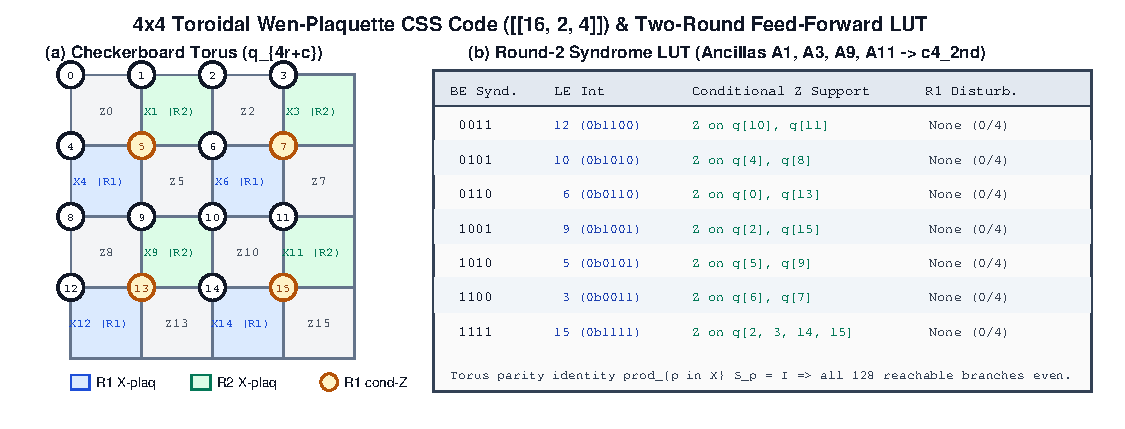
\includegraphics[width=\columnwidth]{fig1_torus_checkerboard_lut.pdf}
\caption{$4\times 4$ toroidal Wen-plaquette layout and $7$-entry Round-2 LUT (BE syndrome $\to$ LE \texttt{pytket} condition integer).}
\label{fig:torus}
\end{figure}

\section{Exact 256-Branch Verification and Noise Benchmark}
Exhaustive trajectory enumeration confirms $128$ reachable branches (probability $1/128$ each) and $128$ zero-probability odd-parity branches ($\prod_{p\in X} S_p = I$), preparing fixed $|00\rangle_L$ ($Z_{L,\mathrm{row}0}=Z_{L,\mathrm{col}0}=+1$, $\langle X_L\rangle=0$). Dual-basis C++ \texttt{AerBackend} runs yield $0/512$ ($X$-basis) and $0/256$ ($Z$-basis) parity violations. Table~\ref{tab:bench} and Fig.~\ref{fig:bench} summarize noisy trajectories across seeds $\{11,22,33\}$.

\begin{figure}[t]
\centering
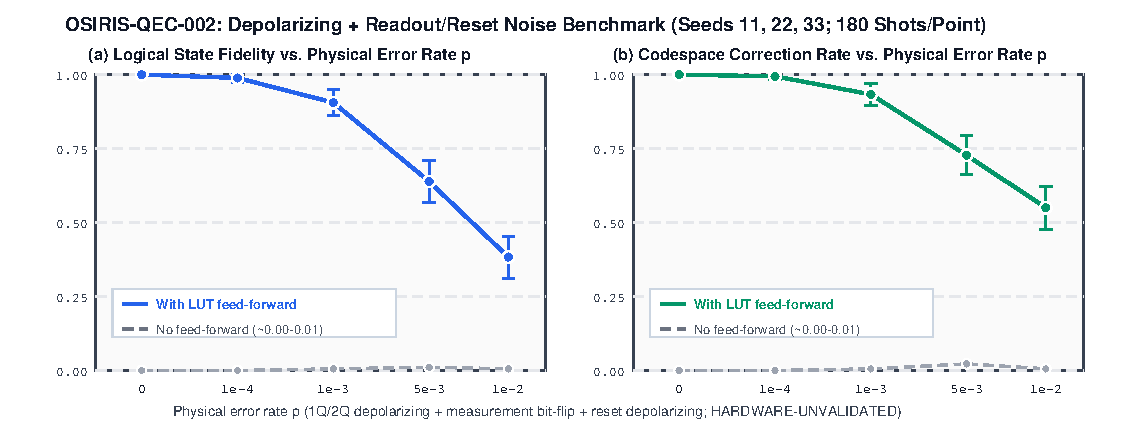
\includegraphics[width=\columnwidth]{fig2_noisy_fidelity_benchmark.pdf}
\caption{Simulated depolarizing + readout/reset noise benchmark ($180$ shots/point) with and without LUT feed-forward.}
\label{fig:bench}
\end{figure}

\begin{table}[t]
\centering
\caption{Pooled noisy preparation benchmark (simulation only).}
\label{tab:bench}
\footnotesize
\begin{tabular}{ccccc}
\toprule
$p$ & Shots & FF Fidelity & FF Codespace & No-FF Fid. \\
\midrule
0 & 180 & $1.0000 \pm 0.0000$ & $1.0000 \pm 0.0000$ & $0.0000$ \\
0.0001 & 180 & $0.9889 \pm 0.0153$ & $0.9944 \pm 0.0109$ & $0.0000$ \\
0.001 & 180 & $0.9056 \pm 0.0427$ & $0.9333 \pm 0.0364$ & $0.0056$ \\
0.005 & 180 & $0.6389 \pm 0.0702$ & $0.7278 \pm 0.0650$ & $0.0111$ \\
0.01 & 180 & $0.3833 \pm 0.0710$ & $0.5500 \pm 0.0727$ & $0.0056$ \\
\bottomrule
\end{tabular}
\end{table}

\section{Pre/Post-Preparation Error Taxonomy and H2 Gate}
Pre-preparation weight-$1$ $Z$ errors are corrected $16/16$ times, whereas post-preparation $Z$ faults flip $X$-syndromes ($16/16$ detectable) without correction ($0/16$, fidelity $<10^{-3}$; Fig.~\ref{fig:gate}), confirming this single-shot preparation circuit is not a QEC memory. Offline \texttt{QuantinuumAPIOffline} H2-1 compilation yields depth $19$ and $32$ \texttt{ZZPhase} gates (SHA-256 \texttt{02d5cb72849f9b473c022e68...}), frozen for \texttt{qnexus} 0.51.4 execution under a $95\%$ Wilson lower bound $>0.99$ ($512/512$, $997/1000$, $1989/2000$, $4964/5000$, $9920/10000$).

\begin{figure}[t]
\centering
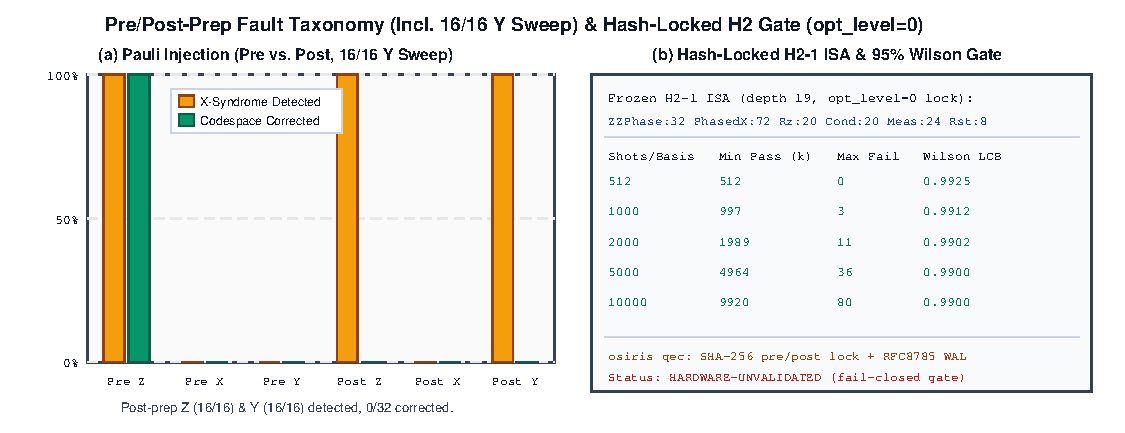
\includegraphics[width=\columnwidth]{fig3_error_taxonomy_and_wilson_gate.pdf}
\caption{Pre- vs.\ post-preparation Pauli injection taxonomy and frozen Quantinuum H2 Wilson ($>0.99$) acceptance gate.}
\label{fig:gate}
\end{figure}

\begin{thebibliography}{9}
\bibitem{Iqbal2024} M. Iqbal \emph{et al.}, Commun.\ Phys.\ \textbf{7}, 205 (2024); arXiv:2302.01917.
\bibitem{Wen2003} X.-G. Wen, Phys.\ Rev.\ Lett.\ \textbf{90}, 016803 (2003).
\bibitem{Kitaev2003} A. Yu. Kitaev, Ann.\ Phys.\ \textbf{303}, 2--30 (2003).
\bibitem{Sivarajah2020} S. Sivarajah \emph{et al.}, Quantum Sci.\ Technol.\ \textbf{6}, 014003 (2020).
\bibitem{Wilson1927} E. B. Wilson, J.\ Am.\ Stat.\ Assoc.\ \textbf{22}, 209--212 (1927).
\bibitem{DavisQEC001} D. P. Davis, OSIRIS-QEC-001, Zenodo \texttt{10.5281/zenodo.24293756} (2026).
\end{thebibliography}
\end{document}
